In \cite{Teachlet} wird die effektive Berechnung der Masse Matrix mit einem Vektor vorgestellt. Diese Methodik sollten wir uns kurz vor Augen führen und daraufaufbauend um einige eigene Gedanken erweitern um diese Methodik für unsere Anwendung zugänglich zu machen.
Das Ziel dieses Unterkapitels ist die Tensorstruktur für die Massematrix und der Laplace Bilinearform herzuleiten und für die Berechnung der Pseudoinversen zu nutzen. 

\subsubsection{Berechnung der Elementmassenmatrix}
Es sei $T$ die Referenzzelle für Rechtecke und $\varphi_i(\bold{x})$ Basisfunktion des diskreten Raumes $V_n$ mit $\bold{x}=(x,y)$ .
\begin{equation} \label{eq:mass}
M_{ik} = \int\limits_{T} \varphi_i (\bold{x}) \, \varphi_j (\bold{x}) \, d\bold{x}
\end{equation}

Die Basisfunktionen haben eine Tensorstruktur, die wie folgt aussieht
\begin{equation} \label{eq:tensor}
\varphi_i(\bold{x})=\varphi_{i_1+(N+1)i_2}(x,y)=\varphi_{i_1}(x)\varphi_{i_2}(y)
\end{equation}

Wir werden eine lexikographische Ordnung der Freiheitsgrade benutzen. Die Reichweite von $\, \, i_1 $ und $ i_2 \, $ reicht von $0$ bis $N$. Das heißt der Index $i$ geht von $0$ bis $N_p=(N+1)^2-1$. In Abbildung (\ref{fig:lexi}) sehen Sie ein Beispiel für $N=3$.

\begin{figure}[ht] 
	\centering
  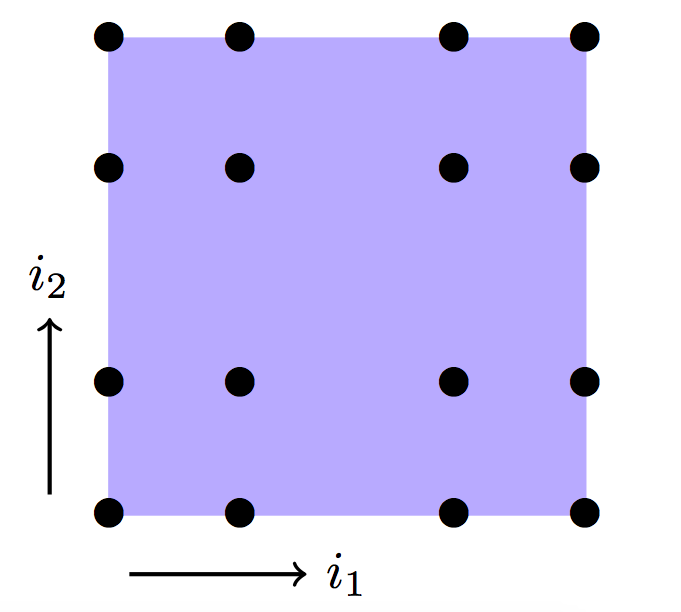
\includegraphics[width=0.3\textwidth]{lexi.png}
	\caption{ \cite[3]{Teachlet}}
	\label{fig:lexi}
\end{figure}

Wir wollen für die Berechnung der Integrale in (\ref{eq:mass}) die Gauss Quadratur benutzen.
Es seien $\bold{x}_q=(x_{q1},x_{q2})$ die Stützstellen und $\bold{w}_q=w_{q1}w_{q2}$ die Gewichte. Dann können wir (\ref{eq:mass}) approximieren wie folgt

\begin{equation} \label{eq:massapprox}
\begin{aligned}
M_{ij} &= \int\limits_{T} \varphi_i (\bold{x}) \, \varphi_j (\bold{x}) \, d\bold{x} \\
&\approx  \sum\limits_{q=1}^Q \bold{w}_q \, \, \varphi_i (\bold{x}_q) \, \varphi_j (\bold{x}_q) \\
&= \sum\limits_{q_1=1}^{Q_{1D}} \sum\limits_{q_2=1}^{Q_{1D}} \varphi_{i_1}(x_{q1}) \varphi_{i_2}(x_{q2}) \varphi_{j_1}(x_{q1}) \varphi_{j_2}(x_{q2}) \, w_{q1} w_{q2}
\end{aligned}
\end{equation}

Wir wählen die Anzahl der Quadraturpunkte $Q_{1D}$ per Dimension so, dass wir exakt integrieren. Wir wählen $Q_{1D}$ gleich der Anzahl der Basisfunktionen $N+1$, da wir mit der Gauss Quadratur mit $N+1$ Stützstellen bis $2N+1$ exakt integrieren und der höchste Grad bei uns $2N$ ist.

Wir definieren uns $\mathcal{N}_{iq}=\varphi_i(x_q)$ und weiterhin die Matrix $\mathcal{W}_{ii}=\bold{w}_i$, die in der Diagonalen die Quadraturgewichte hat und sonst Nullen. Damit können wir nun die Massematrix schreiben als
\begin{equation}
M = \mathcal{N} \mathcal{W} \mathcal{N}^T
\end{equation}

Dies ist die Form mit in $\mathcal{N}$ an Stützstellen evaluierte zweidimensionale Basisfunktionen. Wir können dies aber weiter aufspalten in eindimensionale Basisfunktionen und dadurch eine Effizienzsteigerung erzielen bei der Berechnung des Matrix-Vektor Produkts mit der Elementmassenmatrix.
\subsubsection{Berechnung der Elementmassenmatrix-Vektor Produkt}

Das Ziel dieses Unterkapitels ist die effiziente Berechnung des Matrix-Vektor Produkts $Mu=v$ mit $M$ als Massematrix.

Wir fangen damit an, die Matrix $\mathcal{N}$ in ein Tensorprodukt aufzuspalten. 
\begin{equation} \label{eq:onedim}
\mathcal{N} = \mathcal{N}^{1D} \otimes \mathcal{N}^{1D}
\end{equation}

Die Matrix $\mathcal{N}^{1D}$ ist nun äquivalent definiert wie $\mathcal{N}$ bloß mit eindimensionalen Basisfunktionen. Äquivalent ausgeschrieben sieht die Gleichung (\ref{eq:onedim}) wie folgt aus

\begin{equation*}
\begin{bmatrix}
\varphi^{2D}_1(\bm{x}_1) & \hdots & \varphi^{2D}_N(\bm{x}_1) \\
\vdots & \ddots & \vdots \\
\varphi^{2D}_1(\bm{x}_Q) & \hdots & \varphi^{2D}_N(\bm{x}_Q)
\end{bmatrix}
=
\begin{bmatrix}
\varphi^{1D}_1(x_1) & \hdots & \varphi^{1D}_n(x_1) \\
\vdots & \ddots & \vdots \\
\varphi^{1D}_1(x_{Q_{1D}}) & \hdots & \varphi^{1D}_n(x_{Q_{1D}})
\end{bmatrix}
\otimes
\begin{bmatrix}
\varphi^{1D}_1(x_1) & \hdots & \varphi^{1D}_n(x_1) \\
\vdots & \ddots & \vdots \\
\varphi^{1D}_1(x_{Q_{1D}}) & \hdots & \varphi^{1D}_n(x_{Q_{1D}})
\end{bmatrix}
\end{equation*}

Wir nutzen absofort $Q_{1D}=N$ und $Q=(N+1)^2$, da wie wir oben bereits argumentiert haben, damit exakt integrieren können.
Wir erinnern uns $v=Mu=\mathcal{N} \mathcal{W} \mathcal{N}^T$. Da $\mathcal{W}$ eine Diagonalmatrix ist, ist es naheliegend diese Multiplikation bereits durchzuführen. Definiere $\mathcal{W}_{N}=\mathcal{N} \mathcal{W}$ und die Spaltung von $\mathcal{W}_N$ sieht wie folgt aus

\begin{equation}
\mathcal{W}_N = \mathcal{W}_N^{1D} \otimes \mathcal{W}_N^{1D}
\end{equation}

Genauer

\begin{equation*}
\begin{bmatrix}
\mathcal{N}_{11} \bold{w}_1 & \hdots & \mathcal{N}_{1N} \bold{w_N} \\
\vdots & \ddots & \vdots \\
\mathcal{N}_{N1} \bold{w}_1 & \hdots & \mathcal{N}_{NN} \bold{w_N}
\end{bmatrix}
= 
\begin{bmatrix}
\mathcal{N}_{11}^{1D} w_1 & \hdots & \mathcal{N}_{1N}^{1D} w_N \\
\vdots & \ddots & \vdots \\
\mathcal{N}_{N1}^{1D} w_N & \hdots & \mathcal{N}_{NN}^{1D} w_N
\end{bmatrix}
\otimes
\begin{bmatrix}
\mathcal{N}_{11}^{1D} w_1 & \hdots & \mathcal{N}_{1N}^{1D} w_N \\
\vdots & \ddots & \vdots \\
\mathcal{N}_{N1}^{1D} w_1 & \hdots & \mathcal{N}_{NN}^{1D}w_N
\end{bmatrix}
\end{equation*}

Damit können wir folgende Umformulierung bereits vornehmen
\begin{equation}
v=Mu= \mathcal{N} \mathcal{W} \mathcal{N}^T= \mathcal{W}_N \mathcal{N}^T =  [(\mathcal{W}_N^{1D} \otimes \mathcal{W}_N^{1D})  (\mathcal{N}^{1D} \otimes \mathcal{N}^{1D})^T]u.
\end{equation}

Mit Lemma (\ref{lemma:transpose}) können wir das Transponieren, wie folgt, reinziehen
\begin{equation}
[(\mathcal{W}_N^{1D} \otimes \mathcal{W}_N^{1D})  (\mathcal{N}^{1D} \otimes \mathcal{N}^{1D})^T]u=
[(\mathcal{W}_N^{1D} \otimes \mathcal{W}_N^{1D})  ((\mathcal{N}^{1D})^T \otimes (\mathcal{N}^{1D})^T)]u.
\end{equation}

Dann nutzen wir Lemma (\ref{lemma:prod}) und erhalten
\begin{equation}
 [(\mathcal{W}_N^{1D} \otimes \mathcal{W}_N^{1D})  ((\mathcal{N}^{1D})^T \otimes (\mathcal{N}_{1D})^T)]u= [(\mathcal{W}_N^{1D} (\mathcal{N}^{1D})^T) \otimes (\mathcal{W}_N^{1D} (\mathcal{N}_{1D})^T)]u.
\end{equation}

\newpage
\subsubsection{Tensorstruktur der Laplace Bilinearform}
Die Formel, leicht geändert, kann benutzt werden um andere Bilinearformen auszudrücken wie die Laplace Bilinearform.  Es sei die Elementsteifigkeitsmatrix der Laplace Bilinearform elementweise gegeben durch

\begin{equation}
V_{ij} = \int\limits_{T} \nabla \varphi_i(\bold{x}) \, \nabla \varphi_j(\bold{x})  d \bold{x}=\int\limits_{T}( \delta_x  \varphi_i(\bold{x})  \delta_x \varphi_j(\bold{x})) + ( \delta_y \varphi_i(\bold{x})  \delta_y \varphi_j(\bold{x})) \, d\bold{x}.
\end{equation}

Wir führen elementare Umformungen durch und nutzen die Linearität des Integrals
\begin{equation}
\begin{aligned}
V_{ij} &= \int\limits_{T}( \delta_x  \varphi_i(\bold{x})  \delta_x \varphi_j(\bold{x})) + ( \delta_y \varphi_i(\bold{x})  \delta_y \varphi_j(\bold{x})) \, d\bold{x} \\ &= \int\limits_{T} \delta_x  \varphi_i(\bold{x})  \delta_x \varphi_j(\bold{x}) d\bold{x} + \int\limits_{T}  \delta_y \varphi_i(\bold{x})  \delta_y \varphi_j(\bold{x}) \, d\bold{x}.
\end{aligned}
\end{equation}

Nun nutzen wir eine Quadratur für das Integral. Es seien $\bold{x}_q=(x_{q1},x_{q2})$ die Stützstellen und $\bold{w}_q=w_{q1}w_{q2}$ die Gewichte, dann folgt für die obere Gleichung

\begin{equation}
\begin{aligned}
V_{ij}  = \sum\limits_{q=1}^{(N+1)^2} \bold{w}_q \delta_x  \varphi_i(\bold{x}_q)  \delta_x \varphi_j (\bold{x}_q) + \sum\limits_{q=1}^{(N+1)^2} \bold{w}_q  \delta_y \varphi_i(\bold{x}_q)  \delta_y \varphi_j(\bold{x}_q) \, .
\end{aligned}
\end{equation}

Wir nutzen nun die Tensorstruktur der Ansatzfunktionen
\begin{equation*}
\begin{aligned}
V_{ij}&=\int\limits_{T}( \delta_x  \varphi_i(\bold{x}) + \delta_y \varphi_i(\bold{x})) ( \delta_x \varphi_j(\bold{x}) + \delta_y \varphi_j(\bold{x})) dx \\ &= \int\limits_{T}( \delta_x  (\varphi_{i1}(x) \varphi_{i2}(y)) + \delta_y (\varphi_{i1}(x) \varphi_{i2}(y)) ( \delta_x ( \varphi_{j1}(x) \varphi_{j2}(y)) + \delta_y  (\varphi_{j1}(x) \varphi_{j2}(y))) dx \\ &= \int\limits_{T}( (\delta_x  \varphi_{i1}(x)) \varphi_{i2}(y) + \varphi_{i1}(x) (\delta_y \varphi_{i2}(y))) ( (\delta_x  \varphi_{j1}(x)) \varphi_{j2}(y) +  \varphi_{j1}(x) (\delta_y \varphi_{j2}(y))) \, dx. \\
\end{aligned}
\end{equation*}

Nun nutzen wir eine Quadratur für das Integral. Es seien $\bold{x}_q=(x_{q1},x_{q2})$ die Stützstellen und $\bold{w}_q=w_{q1}w_{q2}$ die Gewichte, dann folgt für die obere Gleichung

\begin{equation*}
\begin{aligned}
&\int\limits_{T}( (\delta_x  \varphi_{i1}(x)) \varphi_{i2}(y) + \varphi_{i1}(x) (\delta_y \varphi_{i2}(y))) ( (\delta_x  \varphi_{j1}(x)) \varphi_{j2}(y) +  \varphi_{j1}(x) (\delta_y \varphi_{j2}(y))) \, dx \\ &= \sum\limits_{q_1=1}^{Q_{1D}} \sum\limits_{q_2=1}^{Q_{1D}} ( (\delta_x  \varphi_{i1}(x_{q1})) \varphi_{i2}(x_{q2}) + \varphi_{i1}(x_{q1}) (\delta_y \varphi_{i2}(x_{q2}))) ( (\delta_x  \varphi_{j1}(x_{q1})) \varphi_{j2}(x_{q2}) +  \varphi_{j1}(x_{q1}) \\ &(\delta_y \varphi_{j2}(x_{q2}))) w_{q1}w_{q2}
\end{aligned}
\end{equation*}

Wir definieren uns zwei Matrizen $\widehat{\mathcal{W}}^{1D}_N$ und $\widehat{\mathcal{N}}^{1D}$ die ähnlich sind wie $\mathcal{W}^{1D}$ und $\mathcal{N}^{1D}$ mit dem Unterschied, dass diese Matrizen nicht die Ansatzfunktionen evaluieren sondern deren Ableitung.

\begin{equation}
\widehat{\mathcal{N}}^{1D} = 
\begin{bmatrix}
\dfrac{\delta \varphi^{1D}_1(x_1)}{\delta x} & \hdots & \dfrac{ \delta \varphi^{1D}_n(x_1)}{\delta x} \\
\vdots & \ddots & \vdots \\
\dfrac{\delta \varphi^{1D}_1(x_{N})}{\delta x} & \hdots & \dfrac{ \delta \varphi^{1D}_n(x_{N})}{\delta x}
\end{bmatrix}
\end{equation}

Analog definieren uns $\widehat{\mathcal{W}}^{1D}_N$.



\newpage
$(\nabla u, \nabla v)$.
\begin{align}
(\nabla u, \nabla v) &=(\partial_x u,\partial_x v) + (\partial_y u,\partial_y v) \\
					   &=\sum_{i,j} u_{ij} (\varphi_i'(x)\varphi_j(y),\phi'(x)\phi(y)) \\
					   & \ + \sum_{i,j} u_{ij} (\varphi_i(x)\varphi_j'(y),\phi(x)\phi'(y))
\end{align}

Nun werden wir 2 Matrizen  $\mathcal{W}'$ und $\mathcal{N}'$ vorstellen.
Diese Matrizen sind ähnlich zu den oben, aber anstatt die Ansatzfunktionen zu evaluieren, evaluieren sie die Ableitung der Ansatzfunktionen. Die resultierende Form ergibt sich aus:
\[\mathcal{V}=\mathcal{W}' \mathcal{N}'^T \mathcal{U} (\mathcal{W} \mathcal{N}^T)^T +\mathcal{W} \mathcal{N}^T \mathcal{U} (\mathcal{W}' \mathcal{N}'^T)^T\]
Sei $(-\Delta u, v)=-(\partial_{xx} u,v) + -(\partial_{yy} u,v)$.\\
Wir führen $\mathcal{N}''$ ein, was die Werte der 2.Ableitung der Ansatzfunktionen in den Quadraturgewichten speichert. Bemerke, dass die Matrix $\mathcal{W}$ nicht modifziert wurde. Als Resultat erhalten wir
\[\mathcal{V}=-\mathcal{W} \mathcal{N}''^T \mathcal{U} (\mathcal{W} \mathcal{N}^T)^T -\mathcal{W} \mathcal{N}^T \mathcal{U} (\mathcal{W} \mathcal{N}''^T)^T\]


Zusammengefasst erhalten wir für die Masse Matrix die Form
\begin{equation}
M*u = (\mathcal{W} \mathcal{N}^{T}) \otimes (\mathcal{W} \mathcal{N}^{T})*u
\end{equation}

und für die Laplace Bilinearform

\begin{equation}
\mathcal{V}*u = -((\mathcal{W} \mathcal{N''}^{T}) \otimes (\mathcal{W} \mathcal{N}^{T}) - (\mathcal{W} \mathcal{N}^{T}) \otimes (\mathcal{W} \mathcal{N''}^{T}))*u
\end{equation}

DIe Berechnung der Pseudoinversen passiert mit diesem Ansatz quasi on the fly, da wir hier gleich als Ergebnis nicht die Pseudoinverse bekommen, sondern das Matrix Vektor Produkt mit der Pseudoinversen als Matrix.

Für die effiziente Berechnung der Inversen brauchen wir folgendes Ergebnis:
\begin{Bemerkung}
\begin{equation}
(A \otimes B)^{-1} = A^{-1} \otimes B^{-1}
\end{equation}
\end{Bemerkung}

Nun erhalten wir fast direkt unser gewünschtes Ergebnis
\begin{equation}
M^{-1}*u = ((\mathcal{W} \mathcal{N}^{T}) \otimes (\mathcal{W} \mathcal{N}^{T}))^{-1}*u
= ((\mathcal{W} \mathcal{N}^{T})^{-1} \otimes (\mathcal{W} \mathcal{N}^{T})^{-1})*u
\end{equation}

$\mathcal{W} \mathcal{N}^{T} \in \mathbb{R}^{n \times n}$ somit also quadratisch. Das heißt um das Pseudoinverse-Vektor Produkt zu berechnen müssen wir nur eine SVD von einer $n \times n$ Matrix berechnen. Falls uns das zu teuer wird können wir auch eine truncated SVD benutzen. In welchem Komplexitätsbereich wir uns befinden, wird im nächsten Subkapitel angeführt.

Für die Laplace Bilinearform ähnlich:
\begin{equation}
\mathcal{V}^{-1}*u = -((\mathcal{W} \mathcal{N''}^{T}) \otimes (\mathcal{W} \mathcal{N}^{T}) - (\mathcal{W} \mathcal{N}^{T}) \otimes (\mathcal{W} \mathcal{N''}^{T}))^{-1}*u
= -((\mathcal{W} \mathcal{N''}^{T})^{-1} \otimes (\mathcal{W} \mathcal{N}^{T})^{-1} - (\mathcal{W} \mathcal{N}^{T})^{-1} \otimes (\mathcal{W} \mathcal{N''}^{T})^{-1})*u
\end{equation}

Praktisch müssen wir also nur die Inversen von $(\mathcal{W} \mathcal{N''}^{T})$ und von $(\mathcal{W} \mathcal{N}^{T})$ berechnen.

Nun war dies der 2 Dimensionale Fall. Die Erweiterung auf den 3 Dimensionalen Fall ist analog und kann im ``Efficient Evaluation ..... Teachlet'' angeschaut werden.

Zu der Implementierungsstrategie kann man in Kapitel 4 mehr erfahren.






